\section{Experiments and Discussion}
 
\subsection{The Agents}

\begin{enumerate}
    \item \textbf{Random Agent} picks an unseen arm half the times and a random seen arm otherwise.
    \item \textbf{Always New Arm Agent} always picks an unseen arm.
    \item \textbf{Naive UCB Agent} picks a new unseen arm with $p=1\%$ and every other time it picks among the known arms using UCB.
    \item \textbf{Naive Thompson Sampling Agent} picks a new unseen arm with $p=1\%$ and every other time it picks among the known arms using Thompson Sampling.
    \item \textbf{Fair UCB Agent} picks a new unseen arm with $p=1\%$ and every other time it picks among the known arms using UCB while also ensuring $\alpha$-Fairness among known arms.
    \item \textbf{Fair TS Agent} picks a new unseen arm with $p=1\%$ and every other time it picks among the known arms using Thompson Sampling while also ensuring $\alpha$-Fairness among known arms.
    \item \textbf{Surplus Curiosity UCB Agent} picks a new unseen arm with a probability based on the surplus, and every other time it picks among known arms using UCB.
    \item \textbf{Surplus Curiosity TS Agent} picks a new unseen arm with a probability based on the surplus, and every other time it picks among known arms using Thompson Sampling.
\end{enumerate}

\subsection{Environments}

\begin{enumerate}
    \item Uniform Environment
    \item Increasingly Better Environment
    \item Progressively Worse Environment
\end{enumerate}

\subsection{Results}

\subsubsection{Uniform Environment}
\begin{figure}[ht]
    \centering
    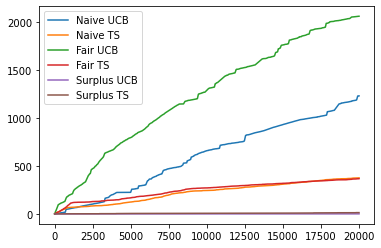
\includegraphics[width=0.8\columnwidth]{static-lin-lin.png}
    \caption{Uniform Environment. Linear-Linear Graph}
    \label{fig:u1}
\end{figure}

\begin{figure}[ht]
    \centering
    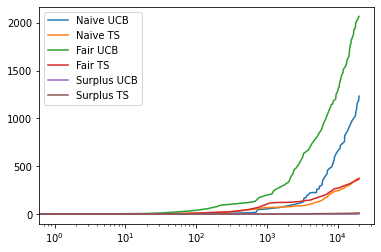
\includegraphics[width=0.8\columnwidth]{static-log-lin.png}
    \caption{Uniform Environment. Log-Linear Graph}
    \label{fig:u2}
\end{figure}

\begin{figure}[ht]
    \centering
    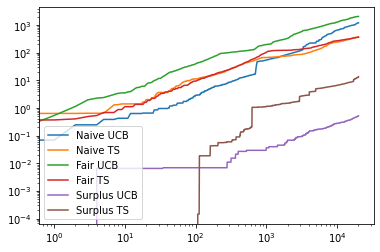
\includegraphics[width=0.8\columnwidth]{static-log-log.png}
    \caption{Uniform Environment. Log-Log Graph}
    \label{fig:u3}
\end{figure}


\subsubsection{Increasingly Better Environment}

\begin{figure}[ht]
    \centering
    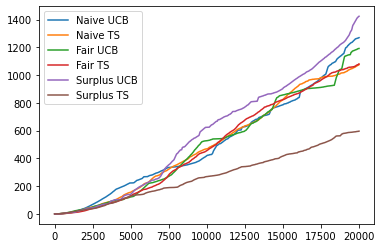
\includegraphics[width=0.8\columnwidth]{inc-lin-lin.png}
    \caption{Increasingly Better Environment. Linear-Linear Graph}
    \label{fig:i1}
\end{figure}

\begin{figure}[ht]
    \centering
    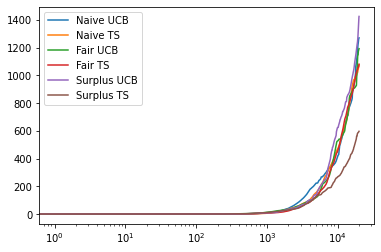
\includegraphics[width=0.8\columnwidth]{inc-log-lin.png}
    \caption{Increasingly Better Environment. Log-Linear Graph}
    \label{fig:i2}
\end{figure}

\begin{figure}[ht]
    \centering
    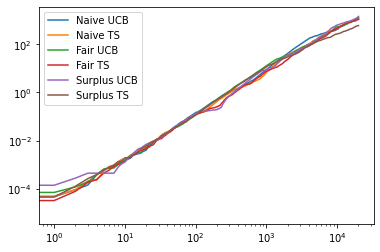
\includegraphics[width=0.8\columnwidth]{inc-log-log.png}
    \caption{Increasingly Better Environment. Log-Log Graph}
    \label{fig:i3}
\end{figure}

\subsubsection{Progressively Worse Environment}

\begin{figure}[ht]
    \centering
    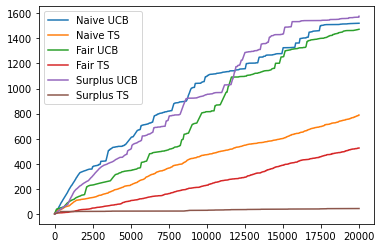
\includegraphics[width=0.8\columnwidth]{dec-lin-lin.png}
    \caption{Progressively Worse Environment. Linear-Linear Graph}
    \label{fig:d1}
\end{figure}

\begin{figure}[ht]
    \centering
    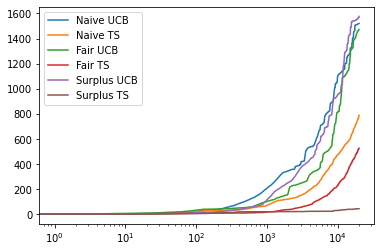
\includegraphics[width=0.8\columnwidth]{dec-log-lin.png}
    \caption{Progressively Worse Environment. Log-Linear Graph}
    \label{fig:d2}
\end{figure}

\begin{figure}[ht]
    \centering
    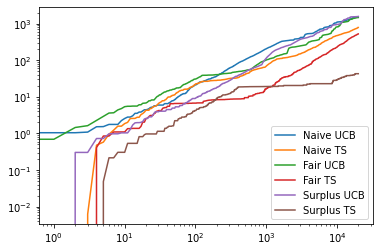
\includegraphics[width=0.8\columnwidth]{dec-log-log.png}
    \caption{Progressively Worse Environment. Log-Log Graph}
    \label{fig:d3}
\end{figure}


\subsection{Discussion}

